\documentclass{article}
\usepackage{fullpage}
\usepackage{amsmath}
\usepackage{graphicx}
\usepackage{hyperref}
\usepackage{verbatim}
\usepackage{pifont}

\begin{document}


\title{Can Evolution Explain Neural Codes?}
\author{Han Kim \ding{41}}
\date{2021 February 10}

\maketitle

\section*{Abstract}

Nervous systems appear efficient. Work from information theory and computer science identify optimal coding schemes across nervous systems, and suggest that evolutionary forces are responsible for the observed efficiency. These claims, however, run counter to tenets of evolutionary biology. Multi-cellular organisms, like those with dedicated neural cell types, are relatively immune to the adaptive power of natural selection. Instead, stochastic non-adaptive forces such as genetic drift and mutational burden are responsible for most of multi-cellular eukaryotic evolution. In this paper, I attempt to reconcile evolutionary biology dogma with the observed efficient coding schemes of biological nervous systems. I propose an overarching evolutionary framework that can accommodate for the prevalence of both optimal and inefficient codes in biology. The apparent incompatibilities between neural and evolutionary-genetic codes arise from biologists' conflation of different organismal `levels'. Evolution can explain the efficiency of neural codes. 

\section{Introduction}

Animals evolve in the absence of strong selection. Population genetics and evolutionary theory show that non-adaptive `neutral' forces are sufficient for explaining coding features at the genomic and cellular levels \cite{Lynch_2007, lynch2007origins}. The explanatory power of such neutral forces increases, as the effective population size of an animal species decreases \cite{Lynch_Conery_2003, kimura1983neutral}. Species with dedicated neuronal cell types are, by definition, multi-cellular eukaryotes, and by this reasoning, evolutionary theory predicts that neutral forces explain the emergence of nervous systems, as well as their functional properties. The overwhelming evidence that many neural coding schemes are efficient appears incompatible with the existing evolutionary biology paradigm \cite{Barlow_2012, Pitkow_Meister_2012, Machens_Gollisch_Kolesnikova_Herz_2005, Mimica_Dunn_Tombaz_Bojja_Whitlock_2018}. In this paper, I examine the basis of this incongruity. I ask whether the efficiency of neural coding demands revisions to the established principles of evolutionary biology, or if it remains under the purview of the field as is.

I begin with a review of non-adaptive evolution and its success in explaining the functional and structural properties of genetic codes. I then survey the contrasting efficiency observed in neural coding. I argue that most modern syntheses of evolution \cite{huxley2010evolution, kimura1983neutral} struggle to explain the efficient coding observed in nervous systems because they fail to provide a satisfactory account of evolution for `higher' phenotypic strata\footnote{Proponents of the recent `Extended Synthesis' \cite{pigliucci2010evolution} might argue otherwise.}. They assume that because genetic information ultimately encodes for physiology and behaviour, that an understanding of how evolution operates at the genetic level also provides an account of how it functions at higher phenotypic levels. I contend that this reasoning is flawed. A rejection of modern evolutionary frameworks' gene-centric overtones can address their inabilities to explain the efficiency of neural codes. Such a modified form of the current evolutionary synthesis properly contextualizes the relative contributions of both non-adaptive and adaptive evolutionary forces, with respect to nervous systems. Evolution explains efficient neural codes. 

\section{Inefficient codes and evolutionary biology}

\subsection{Theory}

Evolution is not natural selection. Rather, it consists of four forces, of which natural selection is just one. The other three---mutation\footnote{Changes to a genetic sequence and is probabilistic, unless engineered.}, recombination\footnote{The swapping of genetic material between sets and is probabilistic, unless engineered.}, and genetic drift\footnote{Changes in a variant's frequency, because of random sampling.}---are non-adaptive because they do not depend on an animal's fitness properties. What factors, then, determine the effectiveness of natural selection on a particular species? The answer to this question will inform an evolutionary biology-oriented hypothesis on how neural codes and nervous systems evolve.

Evolutionary theory and empirical evidence have identified a species' effective population size as the key factor for determining the efficacy of natural selection. In modern evolutionary terms, the effective population size is more concretely expressed as $N_g$, the effective number of inheritable units\footnote{Biological data suggests that genetic material is the unit of inheritance.} in a population\footnote{$N_g$ is a modern variant of the original term for the effective population size, $N_e$. Whereas $N_g$ makes explicit reference to the unit of inheritance, genetic material, $N_e$, as originally conceived by Sewall Wright, does not \cite{wright_1931}. Many methods exist for estimating $N_e$ or $N_g$, each with their own caveats \cite{wang_2016}.}. If we express the efficacy of natural selection as $s$,\footnote{Ronald Fisher first proposed the notion of a selection coefficient \cite{fisher_1930}. Like the effective population size, many methods exist for estimating $s$, each with their own caveats \cite{luis-miguel_2011}.} which when expressed in common terms, is the difference in relative fitness between two alleles\footnote{Alleles are `versions' of an inheritable unit, namely a gene. Gene A with some mutation, \textit{x}, is an allele of gene A.}, we can articulate the efficacy of natural selection\footnote{Drift is $\frac{1}{2N_g}$ for diploid species.} as

\begingroup
\large
\begin{equation}
    \frac{\text{selection}}{\text{drift}} = \frac{s}{\frac{1}{N_g}} = N_g s.
\end{equation}
\endgroup

Classic evolutionary biology theory\cite{kimura1983neutral, Lynch_2007} has shown that the relative contributions of selection and drift, as expressed in equation 1, can be used with the ratio of forward to reverse mutation rates\footnote{The mutation rate of a non-advantageous allele mutating into an advantageous allele, relative to the advantageous allele reverting to the non-advantageous allele.}, $m$, to generate a concrete definition of evolution: 
\begingroup
\large
\begin{equation}
\begin{split}
    \pi & = m e^{2 \frac{\text{selection}}{\text{drift}}} \\
    \pi & = m e^{2N_g s}.
\end{split}
\end{equation}
\endgroup

That is, evolution is the change in frequency of inheritable units over time. $\pi$ is the probability that a beneficial inheritable unit becomes fixed in a population. From this precise definition of evolution, we can substitute different values for the relative contributions of selection and drift, $2N_g s$, such that high values represent natural selection-driven trajectories, and low values represent drift-driven trajectories. A plot of these substitutions (Figure 1) reveals that when natural selection dominates the course of a species' evolution, the probability that an advantageous allele becomes fixed is guaranteed, irrespective of the ratio of forward to reverse mutation rates. Conversely, when drift is the overwhelming evolutionary force---that is, when $\frac{1}{N_g} \gg |s|$---the ratio of forward to reverse mutation rates determines the species' trajectory. In other words, a neutral non-adaptive evolutionary force, mutation, dictates the animal's evolution. We can formalize this evaluation:
\begingroup
\large
\begin{equation}
\begin{split}
    \pi & = \lim_{\frac{1}{N_g} - s \to \infty} m e^{2 \frac{s}{\frac{1}{N_g}}} \\
    \pi &= m e^0 \\
    \pi & = m.
\end{split}
\end{equation}
\endgroup

Given that $N_g$, the effective population size, defines drift and the relative contribution of natural selection on a species' evolution, we can conclude from the above derivations that animals with exceptionally small $N_g$ must be relatively impervious, although not immune, to adaptive evolutionary force. Multi-cellular eukaryotes, like animals with nervous systems, possess small effective population sizes \cite{Lynch_Conery_2003}. In the next section, I examine the explanatory power of non-adaptive forces and evolutionary theory, with respect to observed biological coding properties. 

% This plot is actually slightly off. Something got botched with the equations. 
\begin{figure}[htp]
\centering
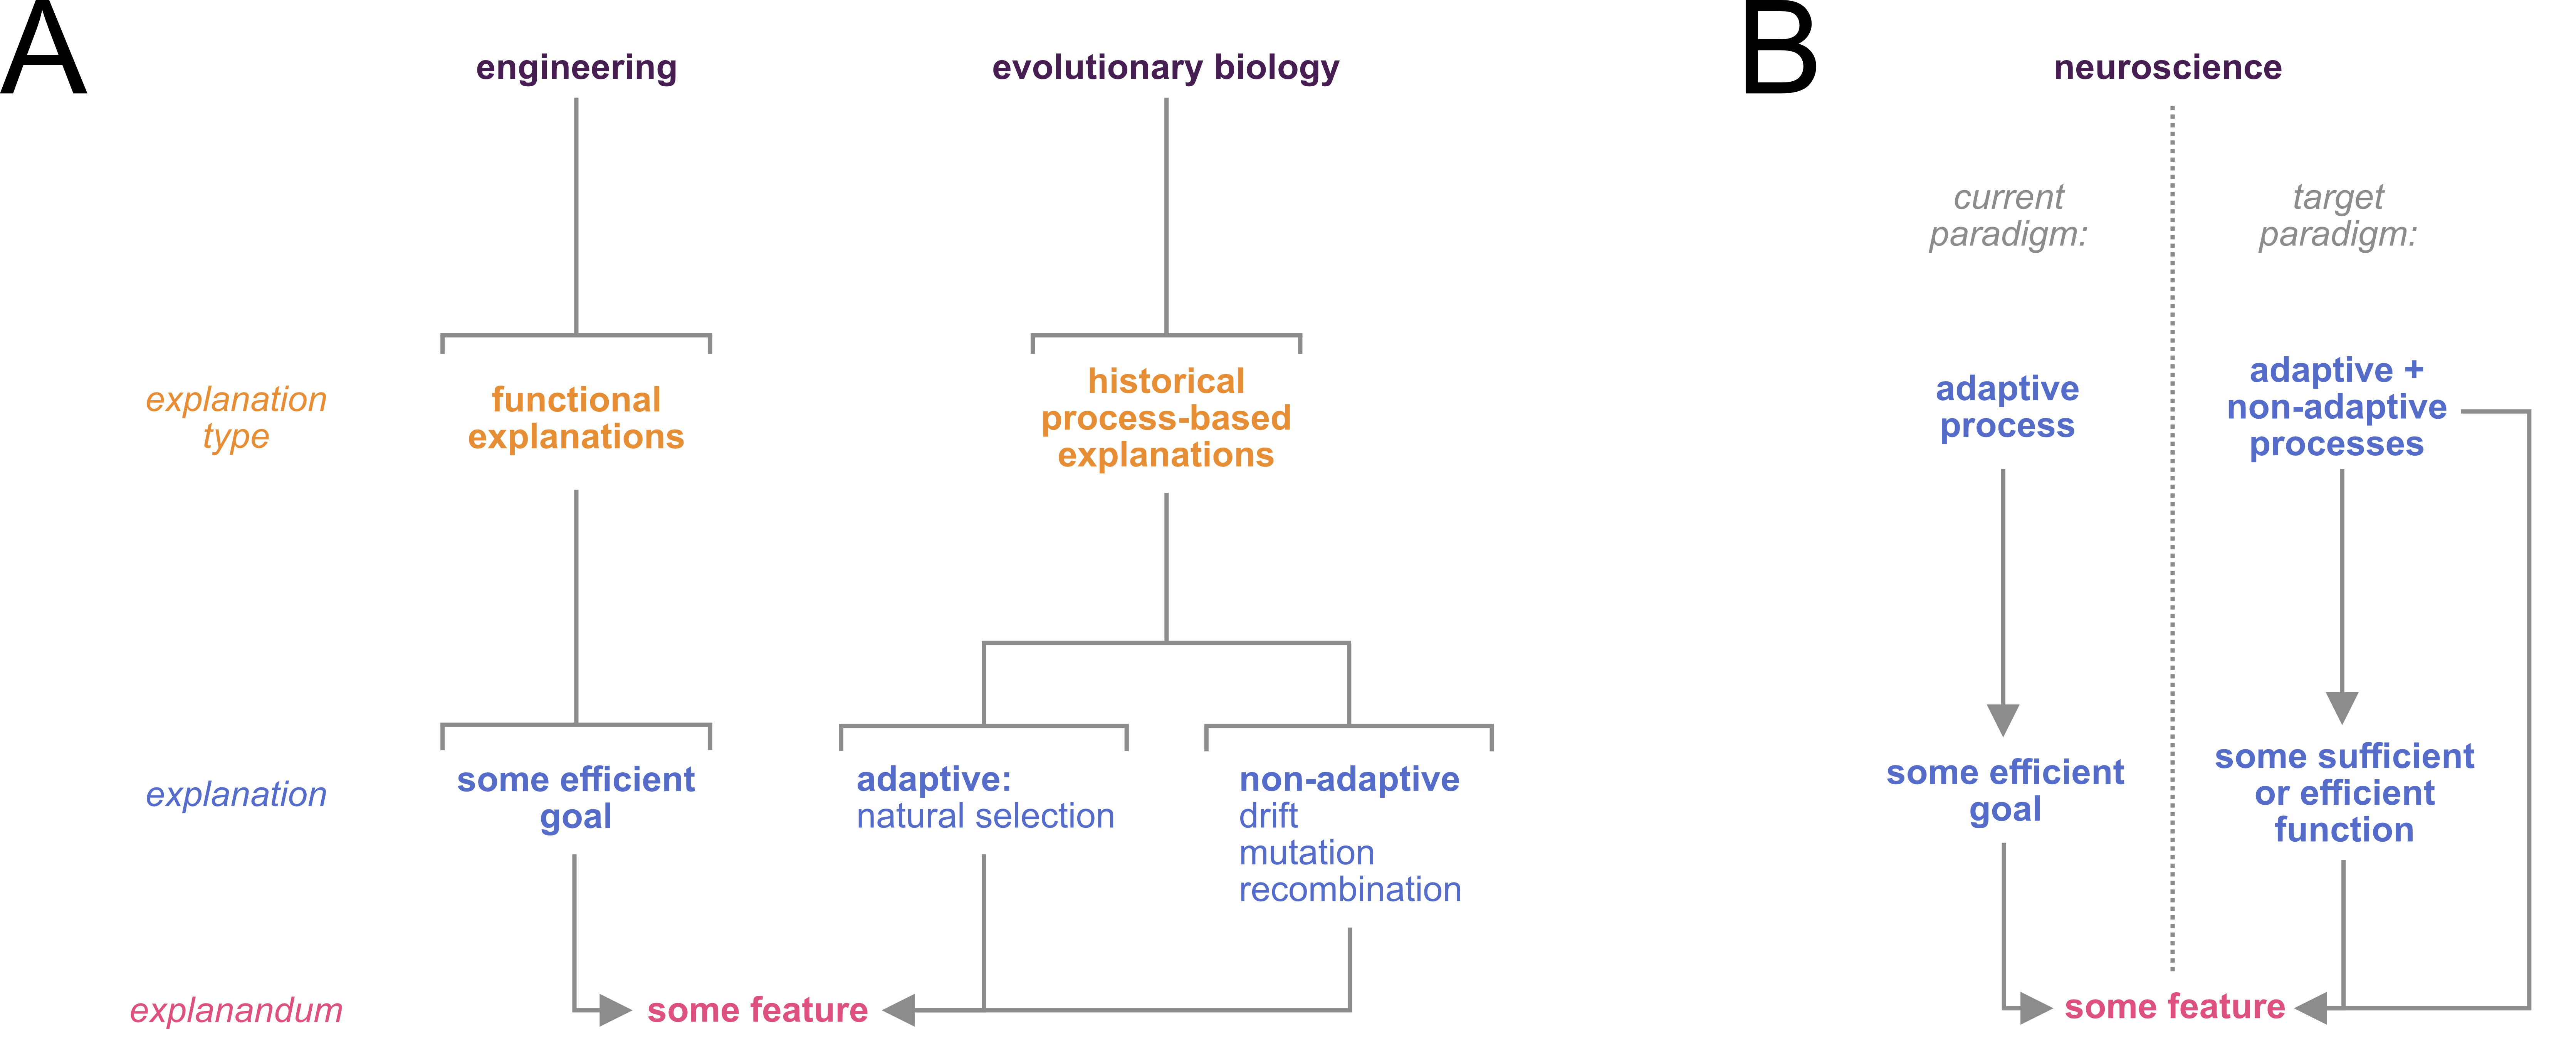
\includegraphics[width=10 cm]{fig_1.png}
\caption{The probability that an advantageous allele in the population reaches fixation, given the allele's selective advantage, $s$, the effective population size, $N_g$, and the ratio of forward to reverse mutation rates, $m$. When $2N_gs=0$, selection does not contribute to the allele's fixation probability, whereas when $2N_gs=\infty$, selection is the exclusive evolutionary force, because the effective population size is infinite. I reproduced this figure based on Lynch 2007 \cite{Lynch_2007}.}
\end{figure}

\subsection{Empirical support for predictions on biological coding efficiency}

Established evolutionary theory predicts that nervous system function should be inefficient, based on the effective population size of multicellular organisms. In animals with small effective populations, beneficial alleles are unlikely to reach fixation. Instead, mutation governs the course of evolution. Given that mutation is a probabilistic process independent of animal fitness, theory predicts that in the absence of strong selection, most mutations are neutral, and we should observe an immense amount of variation and inefficiency across coding elements. Neuroscience should consider this hypothesis seriously, given its abundance of experimental support. 

For one, empirical estimates of effective population sizes\footnote{At this point in the paper, I should clarify the importance of the term ``effective", in the term ``effective population size". The inheritance and population structure of coding elements seen in large populations can sometimes behave like those in small populations, for example, if a minor fraction of individuals contribute to the reproductive pool.}, scaled by the mutation rate, reveal that prokaryotes and unicellular eukaryotes possess the largest estimate of the composite parameter (Figure 2). These species are likely highly susceptible to natural selection. At the opposite end of the scale are multi-cellular organisms, including popular nervous system-possessing laboratory species: \textit{D. melanogaster}, \textit{C. elegans}, and \textit{M. musculus}. Estimates of the effective population size from sequencing data, together with modern evolutionary theory, suggest that nervous system-possessing animals should be weakly subject to adaptive pressures. 

\begin{figure}[htp]
\centering
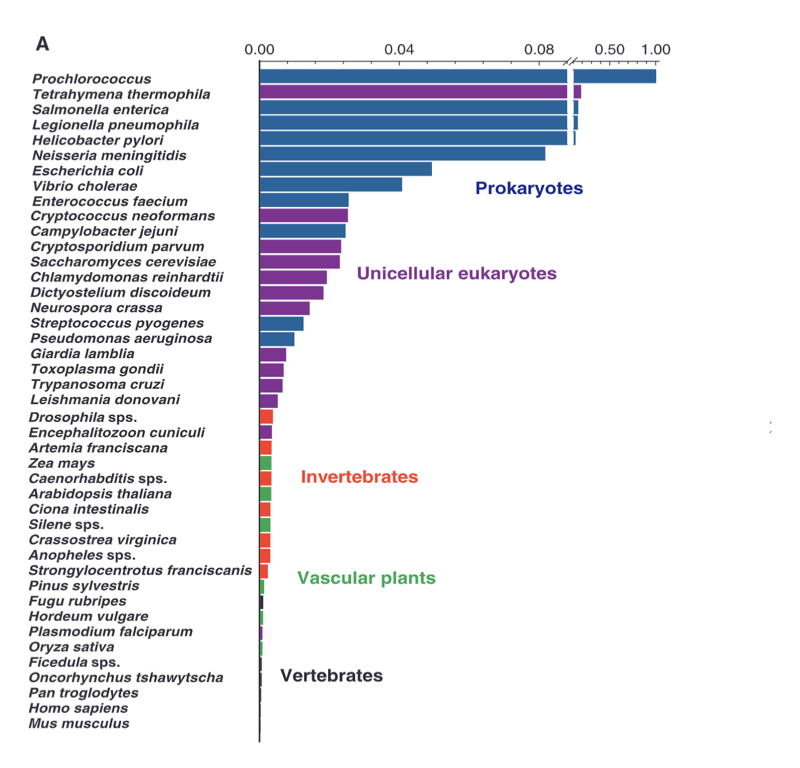
\includegraphics[width=10 cm]{fig_2.jpeg}
\caption{Estimates of $2N_g m$ (x-axis) across a diverse range of species, based on polymorphisms from sequencing data. A facsimile of Figure 1 from Lynch \& Conery, 2003 \cite{Lynch_Conery_2003}.}
\end{figure}

Further evidence for the impact of effective population size on the efficacy of natural selection can be found by analyzing the structural and functional properties of genetic material, the universal biological coding element. The genome architectures of large effective population size species, such as prokaryotes, appear remarkably efficient. Nearly all of their genomes are dedicated to coding proteins and they possess virtually no non-coding sequences, such as introns and non-coding RNA \cite{lynch2007origins, milo2016cell}. In addition, genes that function in common biological processes are found adjacent to each other in the genome, such that the organism can readily achieve co-expression of those related genes \cite{overbeek_matlsev_1999}. Prokaryotic genes can also be polycistronic, meaning that a single mRNA transcript can encode multiple proteins at a time \cite{kozak_1999}. 

In contrast, genetic coding in multicellular eukaryotes appear to be anything but efficient. Eukaryotic genes are monocistronic, and so more energy and molecular machinery must be expended to transcribe and translate a given coding unit \cite{kozak_1999}. Moreover, the majority of multi-cellular eukaryotic genomes are non-coding elements. Less than 2\% of human genes are protein-coding, whereas  90\% to 100\% of prokaryotic genomes encode for functional units \cite{milo2016cell}. The dynamics of coding in multi-cellular organisms is also remarkably inefficient. Most of the eukaryotic genome is transcribed, and yet only a small fraction of those transcripts undergo maturation and subsequent translation into proteins \cite{menet_rosbash_2012}. Transcripts not processed for maturation and translation are digested and decayed \cite{mcnicoll_neugebauer_2014}. The large investment of energy in producing intermediary products from nearly all of the genome, only to have most of those intermediates degraded, illustrates a highly inefficient biological coding process. 

Modern evolutionary theory explains these ideas, without necessarily invoking efficiency and natural selection \cite{lynch2007origins}. Put succinctly, species with small effective population sizes are not subject to strong selective force. Defaulting to a non-adaptive account of evolution circumvents the biologist from hypothesizing untestable and undiscovered objective functions, in the face of sub-optimality. Modern evolutionary theory does not, however, attempt to mitigate the importance of natural selection. As observed in the case of unicellular coding elements, it readily explains efficient codes, when an explanation that appeals to non-adaptive forces alone is insufficient. The current evolutionary paradigm simply articulates under what circumstances we should expect to appeal to natural selection, when explaining biological observations. In the following section, we examine the efficiency of neural codes in the light of evolution, and ask whether such efficiency is expected. 

\section{Efficient codes and nervous systems}

We should not expect efficient neural codes, according to established evolutionary thinking. Nevertheless, the evidence for efficient neural coding is compelling. In feline, human, and grasshopper auditory systems \cite{Machens_Gollisch_Kolesnikova_Herz_2005, smith_lewicki_2006}, sensory neurons appear to use a sparse spike code to represent the acoustic structure of a given stimulus. Kernel functions for an optimal sparse representation learned from auditory stimuli closely approximate the physiological reverse-correlation filters \cite{smith_lewicki_2006}. Importantly, these efficient codes only succeed in using a sparse representation when the auditory stimulus is derived from natural scene statistics. In other words, efficient neural codes appear to at least be correlated with the germane particulars of the animal's natural environment. The exquisite and optimal match between an animal's native environment and the neural code that processes features of that environment tempts a justified invocation of natural selection as an explanation for the observed coding efficiency. This temptation appears further justified, because efficient codes are not only restricted within the ethological sensory space, but are especially tuned for those stimuli that are behaviourally relevant \cite{Machens_Gollisch_Kolesnikova_Herz_2005, machens_herz_2001}. A cohesive and simple explanation of these findings would be that selective forces encompass ethological cues, and animals that fail to efficiently respond to those cues exhibit survival-inappropriate behaviours, and are selected against. In light of an educated evolutionary framework, however, such an explanation, while intuitive, feels conflicting.

We observe theoretical and experimental evidence for efficient neural codes in modalities apart from audition. For example, a survey of ommatidia diameter and eye height from 27 \textit{Hymenoptera} species suggest that their facets have evolved to maximize visual sampling, while minimizing the blur from diffraction \cite{barlow_1952}. This conclusion derives from a fundamental physics principle showing that the optimal resolving power of a lens with diameter $d$ is equivalent to $\sqrt{a \lambda}$, where $a$ is the angle subtended by two point sources that can still be detected as double, and $\lambda$ is the wavelength of incoming light. The surveyed insects indeed possess a linear and proportional relationship between $\sqrt{a}$ and $d$ \cite{barlow_1952}. In terms of neural coding, the retinal ganglion cells of both salamanders and macaques decorrelate spatial features of visual inputs, as a means of achieving sparse spiking in the retina and optimizing visual coding efficiency \cite{Pitkow_Meister_2012}. 

We also find efficiency at the opposite end of the periphery, although not necessarily with respect to neural coding. Instead, most examples of efficient motor control are seen in terms of the amount of energy expended in muscles, to achieve a particular task. Given that the amount of muscle energy required for a behaviour vastly exceeds those needed for neural spiking \cite{sengupta_2010, ortega_2015}, one can argue that the relevant cost function at the motor periphery should relate to the joules of muscle work expended, rather than some sparse spike code. Classic work on horse gaits show that freely moving horses self-optimize their movement speeds. Under naturalistic conditions, they largely operate in locomotor regimes that require minimal amounts of consumed oxygen for moving some unit distance. These results hold across multiple gait types, such as walks, trots, and gallops \cite{hoyt_taylor_1981}. Similar results of self-optimization with respect to gross energy expenditure have also been reported in human ergometer studies \cite{sparrow_newell_1998}. 

Despite the foremost relevance of muscle expenditure over neural spiking for motoric efficiency, some recent evidence suggests that the encoding of naturalistic behaviours may also have some efficient basis. Simultaneous microdrive recordings and 3D posture tracking of the head, neck, and back of freely moving rats reveals that proportionately fewer cells in the posterior parietal and motor cortices fire when the animal partakes in common `default' postures \cite{Mimica_Dunn_Tombaz_Bojja_Whitlock_2018}. The encoding of naturalistic poses appears to use a minimal number of cells to represent the repertoire of ethological motor ensembles. 

Further examples of efficiency are found in other deep processing regions, albeit often with different objectives from the sparse coding seen at the periphery \cite{simoncelli_2003}. Learning algorithms that maximize sparseness, for example, succeed in recapitulating the spatially localized, oriented, and bandpass features of mammalian visual cortical cells \cite{olshausen_field_1996}. In general, sparse codes in the visual cortex appear to be useful for learning and processing incoming spike patterns \cite{olshausen_field_1996}, or for parsing large amounts of signal from background noise \cite{ringach_malone_2007}, in the face of overcomplete representations. Even though these kinds of objective functions differ from those efficient representations seen in the periphery, where the goal is to minimize the number of spikes needed for expressing some maximal description of the environment, both scenarios still offer examples of efficient coding. 

Given the abundance of strong empirical and theoretical work in favour of efficiency in neural codes, modern evolutionary frameworks must address the apparent paradox between the small effective population sizes of nervous system-possessing animals and the efficiencies of neural coding. In the next section, I speculate as to why such a conflict appears to exist. I provide a possible reconciliation of the evidence found across neuroscience and evolutionary biology. 

\section{An account of phenotypic evolution}

Natural selection is relatively inefficient in nervous system-possessing animals. While I maintain this assertion in my forthcoming arguments, I contend that modern evolutionary thinking fails in assuming that the relative contributions of evolutionary forces on the hereditary unit, genetics, extends uniformly and necessarily to the highest levels of phenotype, such as behaviour and neurophysiology. Modern evolutionary frameworks assume that because genetic material ultimately encodes for all biological processes, that by developing and testing theories about the root cause, they are effectively developing theories that are also about the encoded products of the genetics. They assume that their explanations extend to those products, by mere substitution. This gene-centric account of evolution does not hold as such, with respect to the evolution of phenotypes. The central dogma of molecular biology \cite{crick_1970} explains how genetic material encodes for protein products, but it does not explain how those proteins encode for organismal function. Theories about genetic information are not equivalent to theories about phenotypes ultimately derived from genetic information. Even Motoo Kimura, the founder of neutral evolutionary theory, speculated that the relevance of neutral theory is likely minimal, with respect to the evolution of phenotypes \cite{kimura1983neutral, zhang_2018}. 

\begin{figure}[htp]
\centering
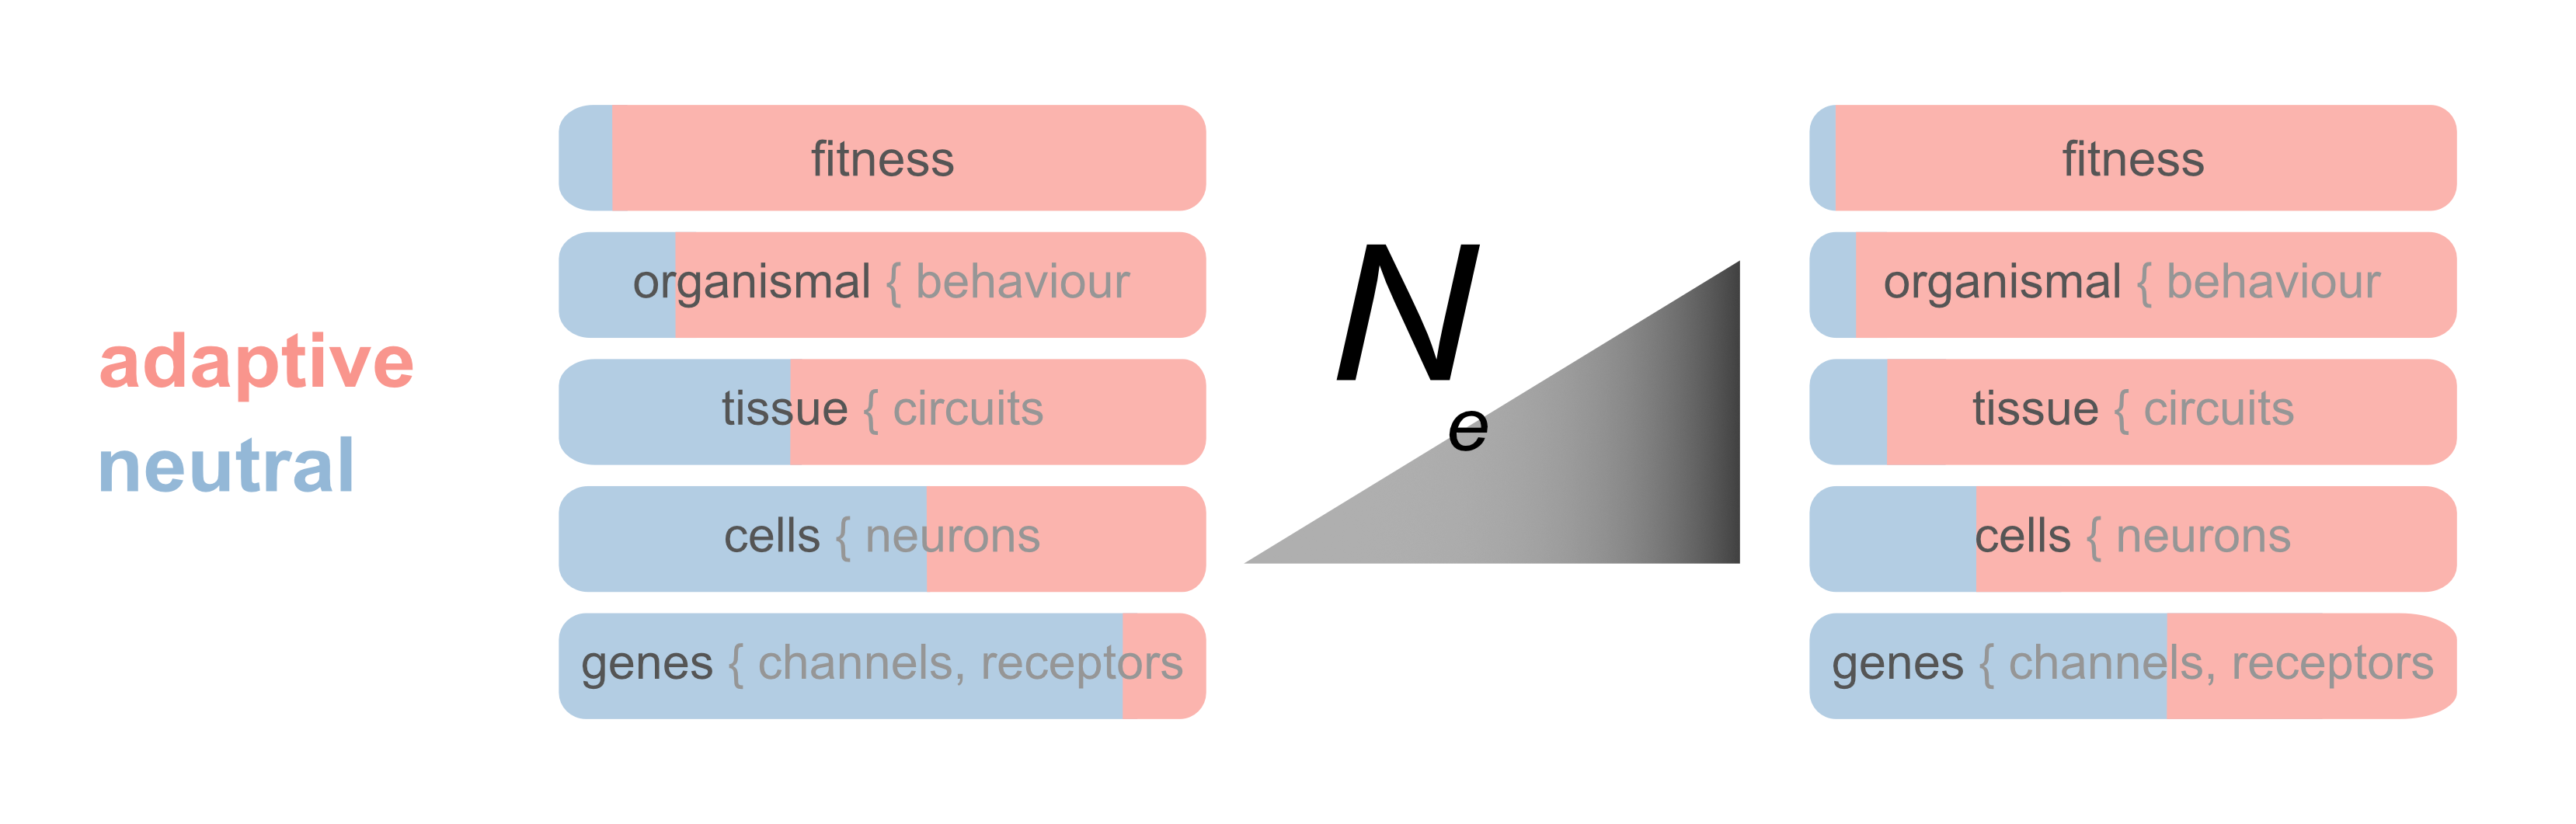
\includegraphics[width=17 cm]{fig_3.png}
\caption{The contribution of neutral and adaptive forces on the evolution of different phenotype levels. Higher phenotype traits are more subject to adaptive forces than traits in lower phenotype levels. The fraction of adaptive changes increases across all phenotype levels as the effective population size increases.}
\end{figure}

We require an amendment to the existing evolutionary framework to account for the evolution of phenotypes. I propose that the divvying of phenotypes into constituent `layers' \cite{Ho_Ohya_Zhang_2017, zhang_2018, wideman_doolittle_2019, mayr_1997} reconciles the efficient codes observed at higher neurophysiological levels with the non-adaptive effects expected at the bottom-most genetic level, for multi-cellular eukaryotes. The key advancement that a hierarchy of `layered' phenotypes provides is that elements of a bottom layer can afford to drift and be inefficient, provided their effects do not impinge on the integrity of the layer directly above. In other words, intermediary layers `buffer' the effects that bottom layers have on the highest layers, such as animal fitness. In contrast, a `layer-free' conception of phenotypes wherein genes directly encode for organismal attributes, results in an unrealisitc and onerous emphasis of the genetic level's impact on species fitness. Such a conception is not compatible with existing biological evidence, because alleles that are slightly deleterious with respect to biochemical and cell-biological levels can exist, without dramatically compromising fitness \cite{wideman_doolittle_2019}. Given that natural selection acts directly on phenotype, rather than genotype, the hierarchical stratification of phenotype, with respect to the genetic level, means that the relative contribution of natural selection on animal evolution is, in fact, a function of two parameters (Figure 3). One is the effective population size, as detailed above. The other is the phenotypic level at which species variation is observed. Such variation can range from the lowest level, genetic material, to the highest levels, such as behaviour and physiology. Change occurring at a level to which selection is blind will be neutral, provided that it does not affect the higher level \cite{mayr_1997, wideman_doolittle_2019, zhang_2018}. By this definition, the probability of a given change being neutral is greater, the lower the level of the change. 

This conception alters the way evolutionary frameworks interpret neural coding phenomena. The efficiency of neural codes can be understood because of its close proximity to the highest level of phenotype. The fact that most efficient neural coding evidence relates to sensory processing---in particular, peripheral sensory processing---as well as the control of naturalistic behaviours, is likely not a coincidence. Neural codes instantiated in these systems interact directly with the native environment, and by extension, with selective forces. Indeed, in the case of the optimal facet angles of \textit{Hymenoptera} ommatidia \cite{barlow_1952}, the efficient implementation is not necessarily neural, but has in common the involvement of an apparatus that routinely interacts with the environment. The relevant parameter that explains the evolution of efficient neural codes is the proximity to phenotype, rather than it being neural, \textit{per se}. For this reason, the proposed framework also applies more broadly to general phenotypic attributes, such as gross animal morphology, and not just to nervous systems. That being said, the intimate relationship between the neural coding of sensory and motor processing, and the features of the external environment, render neural coding architectures unusually susceptible to adaptive evolution.

A consideration of the level of phenotypic change and its proximity to fitness can potentially explain additional neuroscience phenomena, outside of sparse coding schemes. A recent report argues from single-cell sequencing data that the origins of the cerebellum may lie in cell duplication events \cite{kebschull_luo_2020}. Duplication events, such as those commonly found in the genes of eukaryotic genomes, are classic hallmarks of neutral evolution \cite{Stoltzfus_1999, Lynch_2007, lynch2007origins, wideman_doolittle_2019}. In the case of genes, duplicates tend not to have overt advantageous or deleterious effects on any phenotype, and so are considered neutral\footnote{Evidence exists that duplication can encourage organismal complexity via subfunctionalization and neofunctionalization of the ancestral copy's original purpose \cite{dean_thornton_2007, Lynch_2007}.}. Given the relatively large distance between fitness and the phenotype level occupied by cell types that do not directly process environmental features, we might hypothesize that, together with the small effective population size of mammals, that neutral events like cell type duplications are expected. From this example, I must emphasize a key point about the addition of phenotypic `layering' in my thinking about evolution. The effective population size of a species still has a profound impact on its evolution (Figure 3). We must consider both effective population size and the proximity of a given change to the uppermost level of fitness, when generating hypotheses about the relative contributions of evolutionary forces. 

In comparison to the cells of a vertebrate anatomical structure, consider the evolution of invertebrate neurons. Invertebrates possess much larger effective population sizes than vertebrates (Figure 2). Consequently, given that cerebellar cells and invertebrate neurons occupy the same level of phenotype---that of cells---we can expect natural selection to more extensively drive the evolution of invertebrate neurons. Spiking local interneurons in the metathoracic ganglion of locusts, for example, have two fields of neuropilar branches that a single process links together (Figure 4). One of these fields possess numerous fine neurites with relatively uniform diameters, and is located in a ventral area where afferents from a hind leg hair also terminate. The other field possesses sparser more varicose neurites, and is located in a more dorsal area, found alongside the neurites of many leg muscle motor neurons. The majority of the dorsal field are output synapses, although they are also capable of receiving inputs, whereas the ventral field consists mostly of input synapses \cite{watson_burrows_1985}. Indeed, these two fields, both of which belong to a single local interneuron, participate in two completely distinct and compartmentalized functions. This multiplexing of computations across space in a single neuron appears absent from the multi-polar neurons of smaller effective population sized species, such as vertebrates. More recent calcium imaging evidence from \textit{C. elegans} also identify spatially compartmentalized multiplexed computations within a single interneuron, RIA \cite{Hendricks_Ha_Maffey_Zhang_2012} (Figure 4). A consideration of both effective population size and phenotypic level can explain the increased efficiency observed in invertebrate neurons\footnote{One corollary to this point that lies somewhat outside the scope of this paper, but still worth mentioning, is that because invertebrates represent the largest effective population sized species that still possess a nervous system, principles of efficient neural coding and organization are probably best exemplified in invertebrates. This evolutionary biology-informed prediction likely has important consequences for engineering applications.}. 

\begin{figure}[htp]
\centering
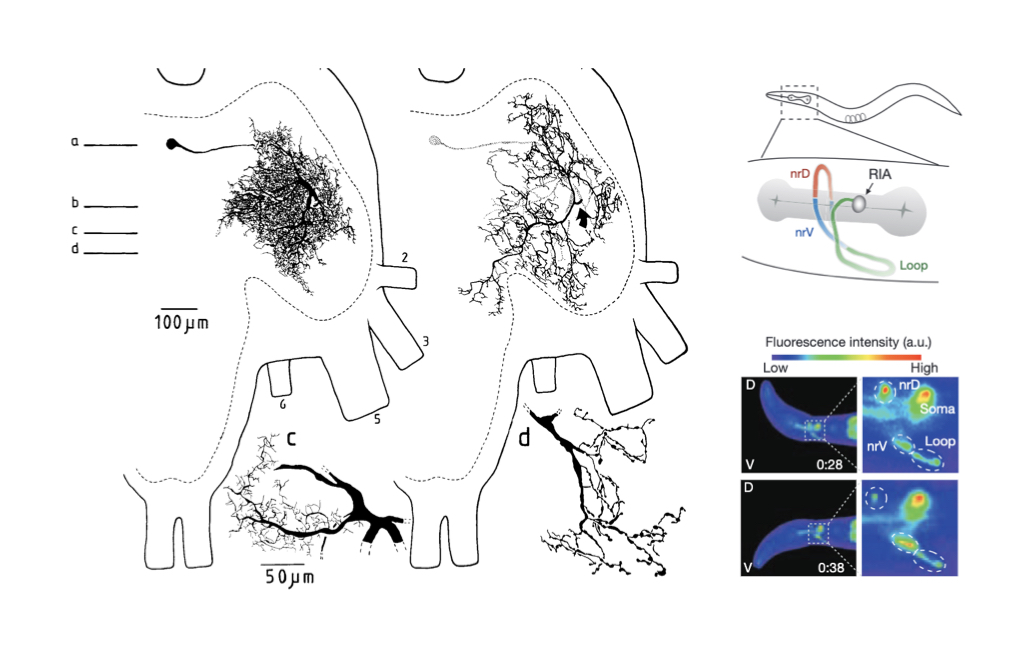
\includegraphics[width=13 cm]{fig_4.jpeg}
\caption{Efficient and multiplexed computations in invertebrate neurons. The left side is a facsimile of Watson and Burrows 1985 \cite{watson_burrows_1985} and depicts the ventral field of a locust interneuron, and to the right of that is the dorsal field of the interneuron. The bottom inset figures are close-ups of the above dorsal and ventral fields. The right side depicts the compartmentalized calcium dynamics of the RIA interneuron in round worms and is a facsimile of Hendricks \textit{et al.} 2012 \cite{Hendricks_Ha_Maffey_Zhang_2012}.}
\end{figure}

In addition to predictions on differing neural coding efficiencies, a phenotypic account of evolution can explain the observed drift or degeneracy of lower level phenotypes, in massively scaled simulations of neuronal networks. The simulation of more than 20 million models of the crab stomatogastric ganglion pyloric rhythm reveals that several disparate biophysical parameters can achieve pyloric-like rhythms. Similar to the bottom-most level of genetic material, biophysical circuit parameters can also drift, provided they accomplish the same higher level phenotype---in this case, the network architecture---required for organismal function and species fitness. This example demonstrates the importance of stratifying phenotypes, in a more neuroscientific context, outside of genetic coding. Natural selection is increasingly blind to bottom layer changes, which are effectively neutral. A clear difference exists between changes proximal to the highest level of phenotype, from those at the lower layers, with respect to the efficacy of natural selection. 

We close with a return to efficient coding in a non-neuroscientific context. Earlier, I outlined the efficient coding architectures of the prokaryotic genome, relative to its multi-cellular eukaryotic counterparts. In the light of an evolutionary framework that stratifies phenotype, these efficiency differences in genetic coding remain sensible. Unicellular organisms, like prokaryotes, not only possess large effective population sizes, but also lack higher-order structures, such as tissues and organs. For these species, the level of genetic coding lies far more proximal to fitness than it does for multi-cellular eukaryotes. We must consider both effective population size and the phenotypic level of change, when assessing the evolutionary forces responsible for derived features. 

% Masatoshi Nei's observations about OR genes are interesting.

\section{Conclusion}
% We cannot propose fundamental principles of neuroscience without first attempting to falsify those principles. If we suspect that a unique set of properties separates neuroscience from its sister biological disciplines, we must ask whether those properties are, in some capacity, unique to the neural sciences. In this paper, I make a serious attempt to apply this treatment to two such proposed principles---efficiency, and by extension, adaptation---by testing the limits to which those principles fit non-neuroscientific phenomena in biology. 
The efficient coding of neural systems is unexpected, in the light of consensus evolutionary biological thinking. Modern evolutionary frameworks predict that the small effective population sizes of nervous system-possessing animals will result in those animals having inefficent neural codes, because of their relative immunity to natural selection. Empirical evidence from neuroscience, however, appears to disprove such a prediction \cite{smith_lewicki_2006, olshausen_field_1996, Machens_Gollisch_Kolesnikova_Herz_2005, Pitkow_Meister_2012, barlow_1952, fairhall_deRuyterVan_2001}. I argue that the reason for this discrepancy is because many evolutionary frameworks fail to properly consider the richness of species phenotypes. They conflate what it means for something to be an object \textit{of} selection, versus an object \textit{for} selection \cite{sober1993nature, mayr_1997}. A conceptual stratification of phenotypes suggests that the proximity to fitness of a phenotypic level is an orthologous axis, in addition to effective population size, that determines the relative contribution of natural selection on an observed biological feature. 

The incorporation of both phenotypic level and effective population size in the evolution of neural systems not only explains seemingly disparate observations in neuroscience, but informs a conceptual framework under which we can devise hypotheses about the evolutionary origins of biological observations. For example, recent findings argue for brainwide representations of ongoing states and behaviours in vertebrates \cite{stringer_harris_2019, allen_deisseroth_2019}. Current thinking interprets these findings in a teleological context, even though such representations appear to exhibit anything but a reduction in redundancy \cite{kaplan_zimmer_2020}. Under a phenotypic account of evolution, however, we should consider the possibility that in small effective population sized species, and in brain regions that do not directly interact with the environment, an appeal to stochastic evolutionary forces is reasonable. It provides basis to earlier thought experiments that questioned the unregulated application of selectionist `just-so' stories in evolutionary biology  \cite{Gould_Lewontin_1979}.

A final point to address is that non-teleological accounts of evolution can be `countered' by the possibility that observed inefficiencies are actually the byproduct of an optimization for some not yet discovered objective function. This refutation is unfalsifiable. I argue for a more measured approach that considers both adaptive and non-adaptive evolutionary forces, and provides two tangible parameters for thinking about the relative contributions of each. 

Neural science is unique in that its coding schemes tend to exist close to the highest phenotypic levels. In this way, the origins of many observations in neuroscience can perhaps be explained with an appeal to natural selection, even though animals with nervous systems possess relatively small effective population sizes. I conclude, however, that although a thoughtless and automated appeal to natural selection may often not prove incorrect when thinking about the origins of many neurobiological features, a careful consideration of all evolutionary forces has, in fact, more explanatory power. Efficiency likely exists in a more pervasive way in neuroscience than in other disciplines of biology, but a full-bodied evolutionary treatment still proves more useful. Evolution can explain neural codes. 

\newpage
\bibliographystyle{plain} 
\bibliography{bibliography.bib}

% \newcommand{\quickwordcount}[1]{%
%   \immediate\write18{texcount -1 -sum -merge -q #1.tex output.bbl > #1-words.sum }%
%   \input{#1-words.sum} words%
% }

% \quickwordcount{main}

\end{document}

